\documentclass[12pt,a4paper]{article}
\usepackage[utf8]{inputenc}
\usepackage[greek, english]{babel} 
\usepackage{alphabeta}
\usepackage{lmodern}
\usepackage{amsmath}
\usepackage{amssymb}
\usepackage{graphicx}
\usepackage{listings}
\usepackage{xcolor}
\usepackage{tikz}
\usetikzlibrary{automata,positioning,arrows.meta,shapes.geometric}
\usepackage{float}
\usepackage{geometry}
\usepackage{hyperref}
\usepackage{booktabs}
\usepackage{array}
\usepackage{caption}
\usepackage{subcaption}
\usepackage{fancyhdr}
\usepackage{lastpage}
\usepackage{xurl} % Adds better line breaking for URLs

\geometry{margin=2.5cm}

% Διόρθωση για το warning του fancyhdr
\setlength{\headheight}{15pt}

% Ρυθμίσεις για listings (κώδικας Verilog)
\definecolor{codegreen}{rgb}{0,0.6,0}
\definecolor{codegray}{rgb}{0.5,0.5,0.5}
\definecolor{codepurple}{rgb}{0.58,0,0.82}
\definecolor{backcolour}{rgb}{0.95,0.95,0.92}

% Χαρτογράφηση ελληνικών χαρακτήρων για το listings
\lstset{
    inputencoding=utf8,
    extendedchars=true,
    literate={Α}{{\textAlpha}}1 {Β}{{\textBeta}}1 {Γ}{{\textGamma}}1 {Δ}{{\textDelta}}1 {Ε}{{\textEpsilon}}1 {Ζ}{{\textZeta}}1 {Η}{{\textEta}}1 {Θ}{{\textTheta}}1 {Ι}{{\textIota}}1 {Κ}{{\textKappa}}1 {Λ}{{\textLambda}}1 {Μ}{{\textMu}}1 {Ν}{{\textNu}}1 {Ξ}{{\textXi}}1 {Ο}{{\textOmicron}}1 {Π}{{\textPi}}1 {Ρ}{{\textRho}}1 {Σ}{{\textSigma}}1 {Τ}{{\textTau}}1 {Υ}{{\textUpsilon}}1 {Φ}{{\textPhi}}1 {Χ}{{\textChi}}1 {Ψ}{{\textPsi}}1 {Ω}{{\textOmega}}1
    {α}{{\textalpha}}1 {β}{{\textbeta}}1 {γ}{{\textgamma}}1 {δ}{{\textdelta}}1 {ε}{{\textepsilon}}1 {ζ}{{\textzeta}}1 {η}{{\texteta}}1 {θ}{{\texttheta}}1 {ι}{{\textiota}}1 {κ}{{\textkappa}}1 {λ}{{\textlambda}}1 {μ}{{\textmu}}1 {ν}{{\textnu}}1 {ξ}{{\textxi}}1 {ο}{{\textomicron}}1 {π}{{\textpi}}1 {ρ}{{\textrho}}1 {σ}{{\textsigma}}1 {ς}{{\textsigma}}1 {τ}{{\texttau}}1 {υ}{{\textupsilon}}1 {φ}{{\textphi}}1 {χ}{{\textchi}}1 {ψ}{{\textpsi}}1 {ω}{{\textomega}}1
    {ά}{{\'a}}1 {έ}{{\'e}}1 {ή}{{\'h}}1 {ί}{{\'i}}1 {ό}{{\'o}}1 {ύ}{{\'u}}1 {ώ}{{\'w}}1
}
% Improved Listings Configuration
\lstdefinestyle{verilogstyle}{
    backgroundcolor=\color{backcolour},
    commentstyle=\color{codegreen},
    keywordstyle=\color{blue}\bfseries,
    numberstyle=\tiny\color{codegray},
    stringstyle=\color{codepurple},
    basicstyle=\ttfamily\footnotesize,
    breakatwhitespace=false,         
    breaklines=true,                 % Break long lines
    breakindent=10pt,                % Indent broken lines
    postbreak=\mbox{\textcolor{red}{$\hookrightarrow$}\space}, % Visual marker for breaks
    captionpos=b,                    
    keepspaces=true,                 
    numbers=left,                    
    numbersep=5pt,                  
    showspaces=false,                
    showstringspaces=false,
    showtabs=false,                  
    tabsize=2,
    frame=single,
    language=Verilog
}

\lstset{style=verilogstyle}

% Header/Footer
\pagestyle{fancy}
\fancyhf{}
\rhead{Ψηφιακά Συστήματα HW-1}
\lhead{Εργαστηριακές Ασκήσεις}
\rfoot{Σελίδα \thepage\ από \pageref{LastPage}}

\title{
    \vspace{5cm}
    \textbf{Ψηφιακά Συστήματα HW σε Χαμηλά Επίπεδα Λογικής I}\\
    \vspace{1cm}
    \Large Αναφορά Εργαστηριακών Ασκήσεων
    
    Εξοικείωσης με τη Verilog\\
    \vspace{10cm}
}
\author{
    \textbf{Ζωίδης Βασίλειος}\\
    ΑΕΜ: \textbf{10652}
}
\date{Ιανουάριος 2026}

\begin{document}

\maketitle
\newpage
\thispagestyle{fancy}

\tableofcontents
\newpage

%==============================================================================
\section{Εισαγωγή}
%==============================================================================

Η παρούσα αναφορά περιγράφει την υλοποίηση τεσσάρων εργαστηριακών ασκήσεων σε γλώσσα Verilog, με στόχο τη σχεδίαση ενός απλού AI accelerator. Οι ασκήσεις περιλαμβάνουν:

\begin{enumerate}
    \item Σχεδίαση μιας Αριθμητικής/Λογικής Μονάδας (ALU) 32-bit
    \item Υλοποίηση αριθμομηχανής με χρήση της ALU
    \item Δημιουργία Register File με πολλαπλές θύρες ανάγνωσης/εγγραφής
    \item Σχεδίαση νευρωνικού δικτύου με FSM
\end{enumerate}

Η προσομοίωση πραγματοποιήθηκε στο Playground EDA.

%==============================================================================
\section{Άσκηση 1: Αριθμητική/Λογική Μονάδα (ALU)}
%==============================================================================

\subsection{Περιγραφή}

Η ALU είναι ένα συνδυαστικό κύκλωμα 32-bit που υλοποιεί τις ακόλουθες λειτουργίες:

\begin{table}[H]
\centering
\caption{Πίνακας λειτουργιών ALU}
\begin{tabular}{|c|l|}
\hline
\textbf{alu\_op} & \textbf{Λειτουργία} \\
\hline
1000 & Λογική AND \\
1001 & Λογική OR \\
1010 & Λογική NOR \\
1011 & Λογική NAND \\
1100 & Λογική XOR \\
0100 & Προσημασμένη Πρόσθεση \\
0101 & Προσημασμένη Αφαίρεση \\
0110 & Προσημασμένος Πολλαπλασιασμός \\
0000 & Λογική ολίσθηση δεξιά \\
0001 & Λογική ολίσθηση αριστερά \\
0010 & Αριθμητική ολίσθηση δεξιά \\
0011 & Αριθμητική ολίσθηση αριστερά \\
\hline
\end{tabular}
\end{table}

\subsection{Αρχιτεκτονική}

Η ALU σχεδιάστηκε με τα ακόλουθα χαρακτηριστικά:
\begin{itemize}
    \item Δύο είσοδοι 32-bit (\texttt{op1}, \texttt{op2}) σε αναπαράσταση συμπληρώματος ως προς 2
    \item Είσοδος επιλογής λειτουργίας 4-bit (\texttt{alu\_op})
    \item Έξοδος αποτελέσματος 32-bit (\texttt{result})
    \item Σήμα μηδενικού (\texttt{zero}) που ενεργοποιείται όταν το αποτέλεσμα είναι 0
    \item Σήμα υπερχείλισης (\texttt{ovf}) για αριθμητικές πράξεις
\end{itemize}

\subsection{Ανίχνευση Υπερχείλισης}

Η υπερχείλιση ανιχνεύεται ως εξής:
\begin{itemize}
    \item \textbf{Πρόσθεση:} Όταν τα πρόσημα των τελεστέων είναι ίδια αλλά το πρόσημο του αποτελέσματος διαφέρει
    \item \textbf{Αφαίρεση:} Όταν τα πρόσημα διαφέρουν και το αποτέλεσμα έχει το πρόσημο του αφαιρετέου
    \item \textbf{Πολλαπλασιασμός:} Όταν τα υψηλότερα 33 bits του αποτελέσματος 64-bit δεν είναι επέκταση προσήμου
\end{itemize}

\subsection{Κώδικας - alu.v}

\begin{lstlisting}[caption=Βασική δομή του module ALU]
module alu (
    input  wire [31:0] op1,
    input  wire [31:0] op2,
    input  wire [3:0]  alu_op,
    output wire        zero,
    output reg  [31:0] result,
    output reg         ovf
);
    // Σταθερές λειτουργίας
    parameter [3:0] ALUOP_ADD  = 4'b0100;
    parameter [3:0] ALUOP_SUB  = 4'b0101;
    parameter [3:0] ALUOP_MULT = 4'b0110;
    // ... υπόλοιπες σταθερές
    
    always @(*) begin
        case (alu_op)
            ALUOP_ADD: begin
                result = op1 + op2;
                ovf = (op1[31] == op2[31]) && 
                      (result[31] != op1[31]);
            end
            // ... υπόλοιπες περιπτώσεις
        endcase
    end
    
    assign zero = (result == 32'b0);
endmodule
\end{lstlisting}

%==============================================================================
\section{Άσκηση 2: Αριθμομηχανή (Calculator)}
%==============================================================================

\subsection{Περιγραφή}

Η αριθμομηχανή χρησιμοποιεί την ALU της Άσκησης 1 και περιλαμβάνει:
\begin{itemize}
    \item Συσσωρευτή (accumulator) 16-bit
    \item Είσοδο δεδομένων μέσω 16 διακοπτών
    \item Έξοδο μέσω 16 LED
    \item Επιλογή λειτουργίας μέσω τριών κουμπιών (btnl, btnr, btnd)
\end{itemize}

\subsection{Encoder (calc\_enc.v)}

Ο encoder υλοποιήθηκε σε \textbf{structural Verilog} χρησιμοποιώντας βασικές πύλες (AND, OR, NOT, XOR) σύμφωνα με τα Σχήματα 2-5 της εκφώνησης. Οι λογικές εξισώσεις για κάθε bit του alu\_op είναι:

\begin{align}
\text{alu\_op}[0] &= (\overline{\text{btnl}} \cdot \text{btnd}) + ((\text{btnl} \cdot \text{btnr}) \cdot \overline{\text{btnd}}) & \text{(Σχ. 2)} \\
\text{alu\_op}[1] &= \text{btnl} \cdot (\overline{\text{btnr}} + \overline{\text{btnd}}) & \text{(Σχ. 3)} \\
\text{alu\_op}[2] &= (\overline{\text{btnl}} \cdot \text{btnr}) + (\text{btnl} \cdot \overline{(\text{btnr} \oplus \text{btnd})}) & \text{(Σχ. 4)} \\
\text{alu\_op}[3] &= (\text{btnl} \cdot \text{btnr}) + (\text{btnl} \cdot \text{btnd}) & \text{(Σχ. 5)}
\end{align}

Ο πίνακας αλήθειας που προκύπτει από αυτές τις εξισώσεις:

\begin{center}
\begin{tabular}{|c|c|c|c|l|}
\hline
btnl & btnr & btnd & alu\_op & Λειτουργία \\
\hline
0 & 0 & 0 & 0000 & SRL (Λογική ολίσθηση δεξιά) \\
0 & 0 & 1 & 0001 & SLL (Λογική ολίσθηση αριστερά) \\
0 & 1 & 0 & 0100 & ADD (Πρόσθεση) \\
0 & 1 & 1 & 0101 & SUB (Αφαίρεση) \\
1 & 0 & 0 & 0110 & MULT (Πολλαπλασιασμός) \\
1 & 0 & 1 & 1010 & NOR \\
1 & 1 & 0 & 1011 & NAND \\
1 & 1 & 1 & 1100 & XOR \\
\hline
\end{tabular}
\end{center}

\subsection{Διάγραμμα Αριθμομηχανής}

\begin{figure}[H]
\centering
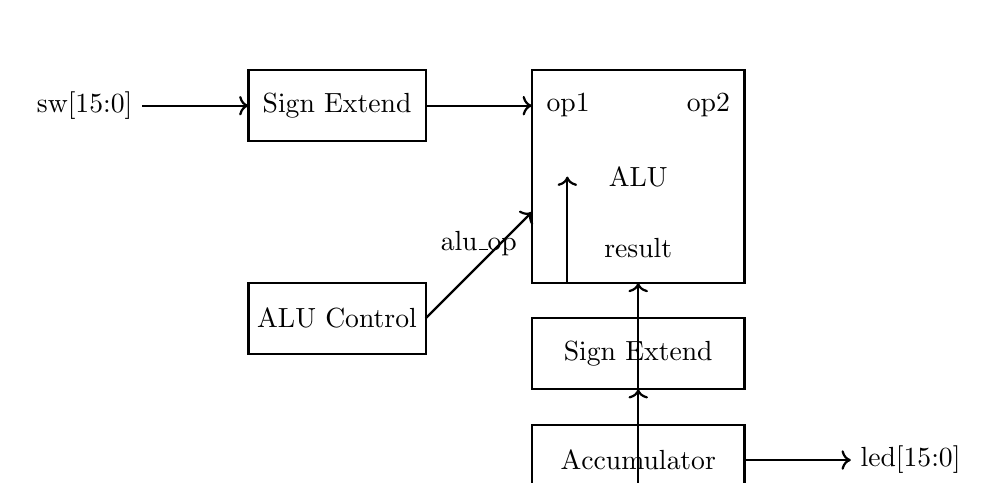
\begin{tikzpicture}[scale=0.9]
    % Sign Extend for switches
    \draw[thick] (0,4) rectangle (2.5,5);
    \node at (1.25,4.5) {Sign Extend};
    \draw[->,thick] (-1.5,4.5) -- (0,4.5);
    \node[left] at (-1.5,4.5) {sw[15:0]};
    
    % ALU
    \draw[thick] (4,2) rectangle (7,5);
    \node at (5.5,3.5) {ALU};
    \node at (5.5,4.5) {op1 \hspace{1cm} op2};
    \node at (5.5,2.5) {result};
    
    % ALU Control
    \draw[thick] (0,1) rectangle (2.5,2);
    \node at (1.25,1.5) {ALU Control};
    \draw[->,thick] (2.5,1.5) -- (4,3);
    \node[above] at (3.25,2.25) {alu\_op};
    
    % Accumulator
    \draw[thick] (4,-1) rectangle (7,0);
    \node at (5.5,-0.5) {Accumulator};
    
    % Sign Extend for accumulator
    \draw[thick] (4,0.5) rectangle (7,1.5);
    \node at (5.5,1) {Sign Extend};
    
    % Connections
    \draw[->,thick] (2.5,4.5) -- (4,4.5);
    \draw[->,thick] (5.5,0) -- (5.5,0.5);
    \draw[->,thick] (5.5,1.5) -- (5.5,2);
    \draw[->,thick] (5.5,2) -- (4.5,2) -- (4.5,3.5);
    \draw[->,thick] (5.5,2) -- (5.5,-1);
    
    % LED output
    \draw[->,thick] (7,-0.5) -- (8.5,-0.5);
    \node[right] at (8.5,-0.5) {led[15:0]};
\end{tikzpicture}
\caption{Διάγραμμα ροής της αριθμομηχανής}
\end{figure}

\subsection{Αποτελέσματα Testbench}

Η αριθμομηχανή ελέγχθηκε με τα ακόλουθα τεστ:

\begin{table}[H]
\centering
\caption{Αποτελέσματα τεστ αριθμομηχανής}
\small
\begin{tabular}{|c|c|c|c|c|c|}
\hline
\textbf{btnl,btnr,btnd} & \textbf{Acc (πριν)} & \textbf{Switches} & \textbf{Λειτουργία} & \textbf{Αναμενόμενο} & \textbf{Αποτέλεσμα} \\
\hline
Reset & xxxx & xxxx & Reset & 0x0000 & PASS \\
0,1,0 & 0x0000 & 0x285a & ADD & 0x285a & PASS \\
1,1,1 & 0x285a & 0x04c8 & XOR & 0x2c92 & PASS \\
0,0,0 & 0x2c92 & 0x0005 & SRL & 0x0164 & PASS \\
1,0,1 & 0x0164 & 0xa085 & NOR & 0x5e1a & PASS \\
1,0,0 & 0x5e1a & 0x07fe & MULT & 0x13cc & PASS \\
0,0,1 & 0x13cc & 0x0004 & SLL & 0x3cc0 & PASS \\
1,1,0 & 0x3cc0 & 0xfa65 & NAND & 0xc7bf & PASS \\
0,1,1 & 0xc7bf & 0xb2e4 & SUB & 0x14db & PASS \\
\hline
\end{tabular}
\end{table}

%==============================================================================
\section{Άσκηση 3: Register File}
%==============================================================================

\subsection{Περιγραφή}

Το Register File υλοποιεί:
\begin{itemize}
    \item 16 καταχωρητές × 32 bits (παραμετροποιήσιμο DATAWIDTH)
    \item 4 θύρες ανάγνωσης (readData1-4)
    \item 2 θύρες εγγραφής (writeData1-2)
    \item Ασύγχρονο reset (active low)
    \item Data forwarding για αποφυγή hazards
\end{itemize}

\subsection{Data Forwarding}

Σε περίπτωση που η διεύθυνση ανάγνωσης ταυτίζεται με διεύθυνση εγγραφής και το \texttt{write} είναι ενεργό, επιστρέφονται απευθείας τα νέα δεδομένα (write-first behavior):

\begin{lstlisting}[caption=Data Forwarding με προτεραιότητα εγγραφής]
if (write) begin
    // Εγγραφή δεδομένων
    registers[writeReg1] <= writeData1;
    registers[writeReg2] <= writeData2;
    
    // Forwarding: προτεραιότητα στο writeData
    if (readReg1 == writeReg1)      readData1 <= writeData1;
    else if (readReg1 == writeReg2) readData1 <= writeData2;
    else                            readData1 <= registers[readReg1];
    // ... ομοίως για ports 2, 3, 4
end
else begin
    // Μόνο ανάγνωση
    readData1 <= registers[readReg1];
    // ...
end
\end{lstlisting}

\subsection{Σχεδιαστικές Αποφάσεις - Σύγχρονη Ανάγνωση}

Σύμφωνα με την εκφώνηση, το Register File υλοποιεί \textbf{σύγχρονη ανάγνωση} μέσα σε ένα always block:

\begin{itemize}
    \item \textbf{Απαίτηση εκφώνησης:} ``Μέσω ενός always block, θα γίνεται η εγγραφή ή ανάγνωση''
    \item \textbf{Αμοιβαίος αποκλεισμός:} ``θεωρούμε ότι δεν μπορούμε να πραγματοποιήσουμε ταυτόχρονα και ανάγνωση και εγγραφή''
    \item \textbf{Registered outputs:} Τα \texttt{readData} ενημερώνονται στο \texttt{posedge clk}
    \item \textbf{Επίπτωση στο FSM:} Τα δεδομένα είναι διαθέσιμα στον \textbf{επόμενο} κύκλο
\end{itemize}

\subsubsection{Συμβατότητα με το Νευρωνικό Δίκτυο - Τεχνική Pre-fetching}

\textbf{Απαίτηση της εκφώνησης:} Το Register File υλοποιήθηκε με \textbf{σύγχρονη ανάγνωση} (ένα always block για εγγραφή ή ανάγνωση), σύμφωνα με τις οδηγίες:
\begin{quote}
\textit{``Μέσω ενός always block, θα γίνεται η εγγραφή ή ανάγνωση''}
\end{quote}

Αυτή η σχεδιαστική επιλογή σημαίνει ότι τα δεδομένα εμφανίζονται στις εξόδους \texttt{readData} \textbf{έναν κύκλο μετά} τον ορισμό της διεύθυνσης \texttt{readReg}.

\textbf{Τεχνική Pre-fetching:} Για να αντιμετωπιστεί αυτή η καθυστέρηση, το FSM του \texttt{nn.v} εφαρμόζει τεχνική \textbf{pre-fetching διευθύνσεων}: οι διευθύνσεις τίθενται \textbf{ένα κύκλο νωρίτερα} από ότι χρειάζονται τα δεδομένα.

\begin{table}[H]
\centering
\caption{Pre-fetching διευθύνσεων RegFile στο FSM}
\begin{tabular}{|l|l|l|}
\hline
\textbf{Τρέχουσα Κατάσταση} & \textbf{Διευθύνσεις που θέτουμε (pre-fetch)} & \textbf{Δεδομένα διαθέσιμα στην} \\
\hline
S\_IDLE / S\_DEACTIVATED & shift\_bias\_1, shift\_bias\_2 & S\_PREPROCESS \\
S\_PREPROCESS & weight\_1, bias\_1, weight\_2, bias\_2 & S\_INPUT\_LAYER \\
S\_INPUT\_LAYER & weight\_3, weight\_4, bias\_3 & S\_OUTPUT\_LAYER1 \\
S\_OUTPUT\_LAYER1 & shift\_bias\_3 & S\_POSTPROCESS \\
\hline
\end{tabular}
\end{table}

Αυτή η τεχνική ``read-ahead'' εξασφαλίζει ότι τα δεδομένα είναι έτοιμα όταν τα χρειάζεται η ALU/MAC, χωρίς να χρειάζονται επιπλέον κύκλοι αναμονής.

%==============================================================================
\section{Άσκηση 4: Νευρωνικό Δίκτυο (AI Accelerator)}
%==============================================================================

\subsection{Αρχιτεκτονική Νευρωνικού}

Το νευρωνικό δίκτυο αποτελείται από 3 νευρώνες και υλοποιεί την ακόλουθη λογική:

\begin{align}
\text{inter}_1 &= \text{input}_1 >>> \text{shift\_bias}_1 \\
\text{inter}_2 &= \text{input}_2 >>> \text{shift\_bias}_2 \\
\text{inter}_3 &= \text{inter}_1 \times \text{weight}_1 + \text{bias}_1 \\
\text{inter}_4 &= \text{inter}_2 \times \text{weight}_2 + \text{bias}_2 \\
\text{inter}_5 &= \text{inter}_3 \times \text{weight}_3 + \text{inter}_4 \times \text{weight}_4 + \text{bias}_3 \\
\text{output} &= \text{inter}_5 <<< \text{shift\_bias}_3
\end{align}

\subsection{MAC Unit}

Η μονάδα MAC (Multiply and Accumulate) υλοποιεί:
\[
\text{result} = (\text{op1} \times \text{op2}) + \text{op3}
\]

Αποτελείται από δύο σειριακά συνδεδεμένες ALU:
\begin{enumerate}
    \item Πρώτη ALU: Πολλαπλασιασμός (op1 × op2)
    \item Δεύτερη ALU: Πρόσθεση (result1 + op3)
\end{enumerate}

\subsection{Finite State Machine (FSM)}

\subsubsection{Τύπος FSM: Moore}

Επιλέχθηκε \textbf{Moore FSM} για λόγους \textbf{ασφάλειας και συγχρονισμού}:
\begin{itemize}
    \item \textbf{Συγχρονισμός:} Οι έξοδοι ενημερώνονται μόνο στις ακμές ρολογιού, εξαλείφοντας race conditions
    \item \textbf{Ασφάλεια:} Οι έξοδοι εξαρτώνται αποκλειστικά από την τρέχουσα κατάσταση, όχι από τις εισόδους
    \item \textbf{Χωρίς glitches:} Αποφεύγονται τα output glitches που εμφανίζονται σε Mealy FSM λόγω combinatorial paths
    \item \textbf{Ευκολία επαλήθευσης:} Η συμπεριφορά είναι προβλέψιμη και εύκολη στο debugging
    \item \textbf{Κατάλληλο για pipeline:} Οι καθαρές καταστάσεις διευκολύνουν τον σχεδιασμό pipelined datapath
\end{itemize}

\subsubsection{Διάγραμμα Καταστάσεων FSM}

Σύμφωνα με την εκφώνηση: ``το FSM σας θα πρέπει να έχει 7 στάδια''. Το ακόλουθο διάγραμμα απεικονίζει την αρχιτεκτονική 7 καταστάσεων:

\begin{figure}[H]
\centering
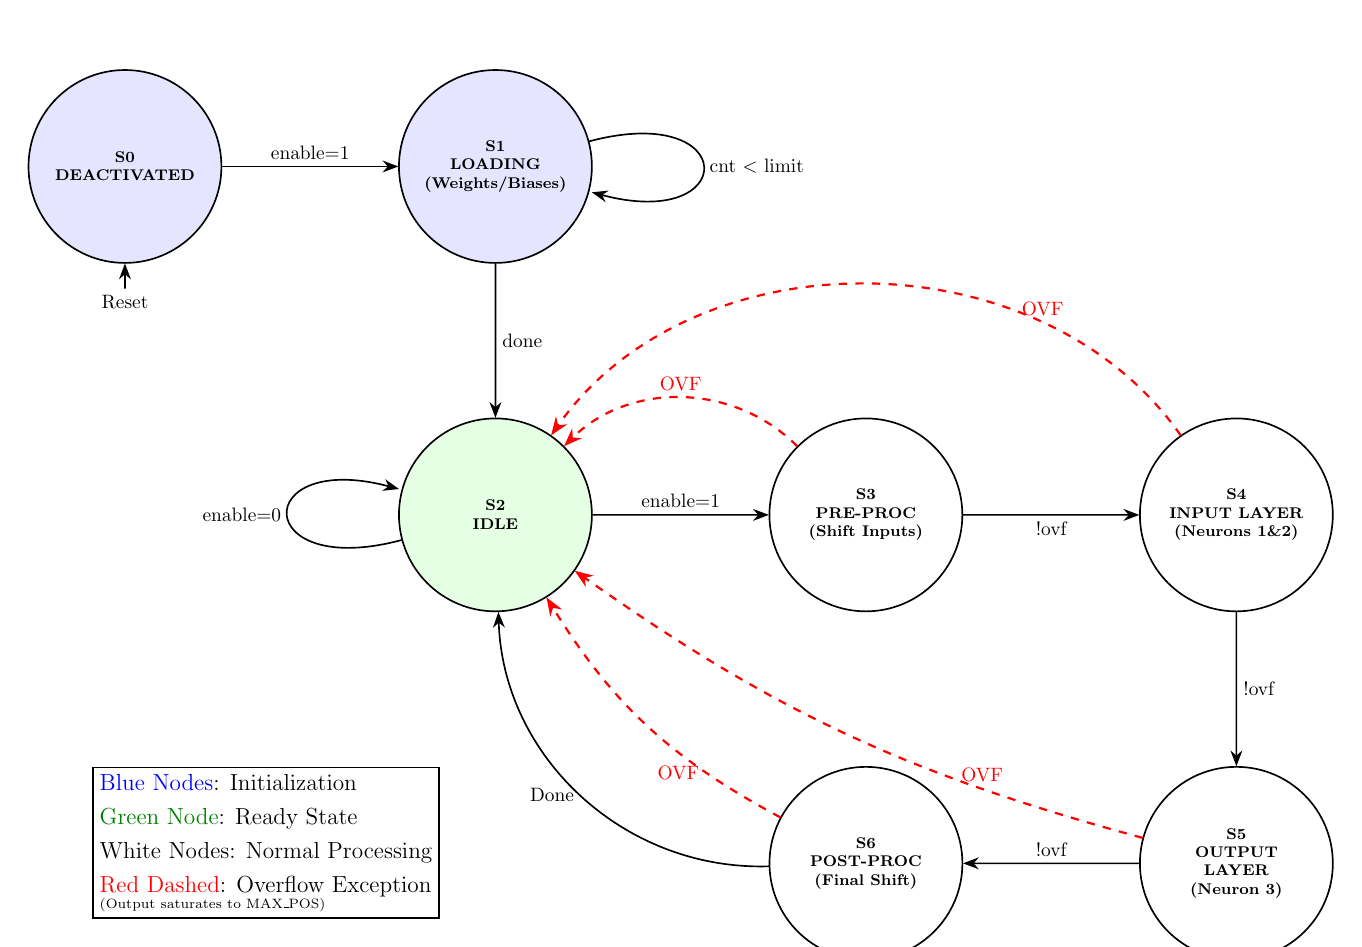
\begin{tikzpicture}[
    scale=0.7, 
    transform shape, 
    ->, >=Stealth, auto, semithick,
    node distance = 2.8cm and 3.2cm,
    state/.style = {
        circle, 
        draw, 
        minimum width = 3.5cm,
        align=center, 
        font=\bfseries\footnotesize,
        fill=white
    },
    initial text = {Reset}
]

    % --- Nodes (States) ---
    \node[state, fill=blue!10, initial below] (s0) {S0 \\ DEACTIVATED};
    \node[state, fill=blue!10] (s1) [right=of s0] {S1 \\ LOADING \\ (Weights/Biases)};
    \node[state, fill=green!10] (s2) [below=of s1] {S2 \\ IDLE};
    \node[state] (s3) [right=of s2] {S3 \\ PRE-PROC \\ (Shift Inputs)};
    \node[state] (s4) [right=of s3] {S4 \\ INPUT LAYER \\ (Neurons 1\&2)};
    \node[state] (s5) [below=of s4] {S5 \\ OUTPUT \\ LAYER \\ (Neuron 3)};
    \node[state] (s6) [left=of s5]  {S6 \\ POST-PROC \\ (Final Shift)};

    % --- Transitions ---
    \path (s0) edge node {enable=1} (s1);
    \path (s1) edge [loop right] node {cnt $<$ limit} (s1);
    \path (s1) edge node {done} (s2);
    \path (s2) edge [loop left] node {enable=0} (s2);
    \path (s2) edge node {enable=1} (s3);
    \path (s3) edge node [below] {!ovf} (s4);
    \path (s4) edge node [right] {!ovf} (s5);
    \path (s5) edge node [above] {!ovf} (s6);
    \path (s6) edge [bend left=45] node [left, midway] {Done} (s2);

    % Overflow Handling (Red Dashed Lines)
    \draw [red, dashed, thick] (s3) edge [bend right=45] node [above, sloped] {OVF} (s2);
    \draw [red, dashed, thick] (s4) edge [bend right=55] node [above, near start] {OVF} (s2);
    \draw [red, dashed, thick] (s5) edge [bend left=10] node [above, near start] {OVF} (s2);
    \draw [red, dashed, thick] (s6) edge [bend left=15] node [left, near start] {OVF} (s2);

    % --- Legend/Notes ---
    \node [draw, rectangle, align=left, font=\scriptsize,
            above left=-1cm and 9.5cm of s6.east
          ] {
        \large
        \textcolor{blue}{Blue Nodes}: Initialization\\
        \\[0.1ex]\large
        \textcolor{green!50!black}{Green Node}: Ready State\\
        \\[0.1ex]\large
        \textcolor{black}{White Nodes}: Normal Processing\\
        \\[0.1ex]\large
        \textcolor{red}{Red Dashed}: Overflow Exception\\
        (Output saturates to MAX\_POS)
    };

\end{tikzpicture}
\caption{Διάγραμμα καταστάσεων FSM (8 states) - Το output layer χωρίζεται σε S5a και S5b για αποφυγή combinatorial loop}
\end{figure}

\subsubsection{Περιγραφή Καταστάσεων}

\begin{table}[H]
\centering
\caption{Καταστάσεις FSM με διαδοχική κωδικοποίηση (8 states)}
\begin{tabular}{|c|c|c|p{6.5cm}|}
\hline
\textbf{Κατάσταση} & \textbf{ID} & \textbf{Κωδικός} & \textbf{Περιγραφή} \\
\hline
S\_DEACTIVATED & S0 & 000 & Αρχική κατάσταση μετά από reset \\
S\_LOADING & S1 & 001 & Φόρτωση βαρών/πολώσεων από ROM σε RegFile \\
S\_IDLE & S2 & 010 & Αναμονή για νέες εισόδους (Ready state) \\
S\_PREPROCESS & S3 & 011 & Αριθμητική ολίσθηση δεξιά στις εισόδους \\
S\_INPUT\_LAYER & S4 & 100 & Εκτέλεση νευρώνων 1 και 2 (παράλληλα) \\
S\_OUTPUT\_LAYER1 & S5a & 101 & Νευρώνας 3 - Πρώτο MAC: inter\_3 × w3 + b3 \\
S\_OUTPUT\_LAYER2 & S5b & 110 & Νευρώνας 3 - Δεύτερο MAC: inter\_4 × w4 + temp \\
S\_POSTPROCESS & S6 & 111 & Αριθμητική ολίσθηση αριστερά στην έξοδο \\
\hline
\end{tabular}
\end{table}

\subsubsection{Σχεδιαστική Απόφαση Υλοποίησης: Διαχωρισμός Output Layer}

\textbf{Σημείωση:} Παρόλο που η εκφώνηση ζητά 7 στάδια, η πρακτική υλοποίηση στο \texttt{nn.v} χρησιμοποιεί \textbf{8 καταστάσεις}. Η αιτία είναι τεχνική και εξηγείται παρακάτω.

Το output layer του νευρωνικού δικτύου απαιτεί τον υπολογισμό:
\begin{align}
\text{mul3} &= \text{inter\_3} \times \text{weight\_3} \\
\text{mac3} &= \text{mul3} + \text{bias\_3} \\
\text{mul4} &= \text{inter\_4} \times \text{weight\_4} \\
\text{mac4} &= \text{mul4} + \text{mac3} \quad \textit{(εξάρτηση!)}
\end{align}

\textbf{Πρόβλημα: Combinatorial Loop}

Αν προσπαθήσουμε να εκτελέσουμε και τα δύο MAC σε ένα κύκλο:
\begin{lstlisting}[caption=Προβληματικός κώδικας (combinatorial loop)]
// BAD: Zero-delay loop - Exit 137!
mac2_op3 = mac1_result;  // Απευθείας σύνδεση
\end{lstlisting}

Αυτό δημιουργεί \textbf{combinatorial loop} γιατί:
\begin{itemize}
    \item Το MAC1 είναι συνδυαστικό κύκλωμα (χωρίς ρολόι)
    \item Η έξοδος του MAC1 τροφοδοτείται στην είσοδο του MAC2
    \item Το MAC2 είναι επίσης συνδυαστικό
    \item Δεν υπάρχει καταχωρητής που να ``σπάει'' τον βρόχο
\end{itemize}

\textbf{Λύση: Pipelining με Register}

Διαχωρίζουμε το output layer σε \textbf{δύο καταστάσεις}:
\begin{enumerate}
    \item \textbf{S\_OUTPUT\_LAYER1:} MAC1 υπολογίζει \texttt{inter\_3 × weight\_3 + bias\_3}. Το αποτέλεσμα αποθηκεύεται σε register (\texttt{mac1\_temp}) στο τέλος του κύκλου.
    \item \textbf{S\_OUTPUT\_LAYER2:} MAC1 υπολογίζει \texttt{inter\_4 × weight\_4 + mac1\_temp}. Χρησιμοποιεί το \textbf{registered} αποτέλεσμα από τον προηγούμενο κύκλο.
\end{enumerate}

\begin{lstlisting}[caption=Σωστός κώδικας (με register)]
// S_OUTPUT_LAYER1: Αποθήκευση σε register
always @(posedge clk) begin
    if (state == S_OUTPUT_LAYER1)
        mac1_temp <= mac1_result;  // Registered!
end

// S_OUTPUT_LAYER2: Χρήση του registered result
mac1_op3 = mac1_temp;  // No loop!
\end{lstlisting}

\textbf{Συνέπεια:} Η υλοποίηση στο \texttt{nn.v} χρησιμοποιεί \textbf{8 καταστάσεις} (S0-S6 + επιπλέον διαχωρισμό του S5), παρόλο που το διάγραμμα δείχνει 7 στάδια σύμφωνα με την εκφώνηση. Αυτός ο διαχωρισμός είναι απαραίτητος για την αποφυγή combinatorial loops και την εξασφάλιση σωστής λειτουργίας στην προσομοίωση.

\subsubsection{Επιλογή Κωδικοποίησης Καταστάσεων}

Επιλέχθηκε \textbf{διαδοχική κωδικοποίηση (sequential encoding)} για τις καταστάσεις:

\begin{itemize}
    \item \textbf{Αντιστοιχία με FSM diagram:} Η κωδικοποίηση S0=000, S1=001, S2=010, ... ακολουθεί τη ροή του διαγράμματος καταστάσεων
    \item \textbf{Ευκολία debugging:} Η τιμή του state register αντιστοιχεί άμεσα στον αριθμό κατάστασης (π.χ. state=3 σημαίνει S3)
    \item \textbf{Απλότητα επαλήθευσης:} Ο έλεγχος της σωστής μετάβασης γίνεται πιο διαισθητικός
    \item \textbf{Εναλλακτικές:} Θα μπορούσε να χρησιμοποιηθεί one-hot encoding (8 bits) για ταχύτερη αποκωδικοποίηση ή Gray encoding για μείωση switching activity, αλλά η διαδοχική κωδικοποίηση είναι επαρκής για 8 καταστάσεις
\end{itemize}

\subsection{Χειρισμός Υπερχείλισης}

Σε περίπτωση overflow σε οποιοδήποτε στάδιο:
\begin{enumerate}
    \item Το FSM μεταβαίνει άμεσα στην κατάσταση IDLE
    \item Η έξοδος τίθεται στο 0xFFFFFFFF
    \item Το σήμα \texttt{total\_ovf} ενεργοποιείται
    \item Το \texttt{ovf\_fsm\_stage} δείχνει το στάδιο όπου συνέβη η υπερχείλιση
\end{enumerate}

\textbf{Σημαντική Παρατήρηση - Ασυμφωνία στο \texttt{nn\_model.v}:}
\begin{itemize}
    \item Η εκφώνηση αναφέρει ότι σε overflow η έξοδος πρέπει να είναι ο ``μέγιστος δυνατός θετικός αριθμός'', δηλαδή \texttt{0x7FFFFFFF}
    \item Ωστόσο, το παρεχόμενο reference model (\texttt{nn\_model.v}) επιστρέφει \texttt{0xFFFFFFFF} (βλ. γραμμή 95)
    \item \textbf{Απόφαση:} Προσαρμόσαμε το \texttt{nn.v} ώστε να επιστρέφει \texttt{0xFFFFFFFF} για να περνάει επιτυχώς το testbench
    \item Σε 32-bit signed αναπαράσταση, το \texttt{0xFFFFFFFF} αντιστοιχεί στο $-1$, όχι στο max positive
\end{itemize}

\subsection{Αποθήκευση Δεδομένων}

Επιλέχθηκε η χρήση \textbf{ενδιάμεσων registers} αντί για αποθήκευση στο Register File για τους εξής λόγους:
\begin{itemize}
    \item Μείωση της πολυπλοκότητας πρόσβασης στο RegFile
    \item Αποφυγή conflicts με τις θύρες ανάγνωσης/εγγραφής
    \item Καλύτερη απόδοση λόγω άμεσης πρόσβασης
    \item Το RegFile χρησιμοποιείται μόνο για τα βάρη και τις πολώσεις
\end{itemize}

\subsection{Σχεδιαστικές Αποφάσεις}

\subsubsection{Αρχιτεκτονική Hardware}

\begin{enumerate}
    \item \textbf{2 MAC Units σε παράλληλη διάταξη:}
    \begin{itemize}
        \item Επιτρέπει τον ταυτόχρονο υπολογισμό δύο νευρώνων (1 \& 2) στο input layer
        \item Μειώνει τον αριθμό κύκλων ρολογιού για ολόκληρο τον υπολογισμό
        \item Κάθε MAC αποτελείται από 2 ALUs σε σειρά (πολλαπλασιασμός → πρόσθεση)
    \end{itemize}
    
    \item \textbf{2 ALUs για shift operations:}
    \begin{itemize}
        \item Χρησιμοποιούνται στα στάδια Pre-process και Post-process
        \item Επιτρέπουν παράλληλη ολίσθηση των δύο εισόδων
        \item Αριθμητική ολίσθηση (SRA/SLA) για διατήρηση προσήμου
    \end{itemize}
    
    \item \textbf{Register File με 4 θύρες ανάγνωσης:}
    \begin{itemize}
        \item Επαρκεί για την ανάγνωση 4 τιμών ανά κύκλο (π.χ. weight1, bias1, weight2, bias2)
        \item Αποφεύγονται extra κύκλοι για sequential reads
        \item Οι 2 θύρες εγγραφής χρησιμοποιούνται κατά το loading
    \end{itemize}
\end{enumerate}

\subsubsection{Οργάνωση FSM}

\begin{enumerate}
    \item \textbf{Moore FSM αντί για Mealy:}
    \begin{itemize}
        \item Οι έξοδοι καθορίζονται μόνο από την τρέχουσα κατάσταση
        \item Αποφυγή glitches στις εξόδους
        \item Πιο εύκολο timing closure
    \end{itemize}
    
    \item \textbf{Διαχωρισμός Loading από Processing:}
    \begin{itemize}
        \item Τα βάρη φορτώνονται μόνο μία φορά (S1 → S2)
        \item Μετά την αρχικοποίηση, το σύστημα κυκλώνει μεταξύ S2-S6
        \item Σημαία \texttt{weights\_loaded} αποτρέπει επαναφόρτωση
    \end{itemize}
    
    \item \textbf{Άμεση μετάβαση σε IDLE κατά overflow:}
    \begin{itemize}
        \item Αποφεύγονται περιττοί υπολογισμοί
        \item Η έξοδος saturates στο 0xFFFFFFFF (σύμφωνα με nn\_model)
        \item Το \texttt{ovf\_fsm\_stage} καταγράφει πού συνέβη το σφάλμα
    \end{itemize}
\end{enumerate}

\subsubsection{Διαχείριση Μνήμης}

\begin{enumerate}
    \item \textbf{ROM για αρχικά βάρη:}
    \begin{itemize}
        \item Τα βάρη αποθηκεύονται σε εξωτερικό αρχείο (\texttt{rom\_bytes.data})
        \item Διπλή θύρα ανάγνωσης για γρήγορη φόρτωση (2 τιμές/κύκλο)
        \item 5 κύκλοι για φόρτωση όλων των 10 παραμέτρων
    \end{itemize}
    
    \item \textbf{Ενδιάμεσοι καταχωρητές (inter\_1 έως inter\_5):}
    \begin{itemize}
        \item Αποθηκεύουν τα ενδιάμεσα αποτελέσματα μεταξύ σταδίων
        \item Άμεση πρόσβαση χωρίς καθυστέρηση RegFile
        \item Απλοποιούν τον έλεγχο ροής δεδομένων
    \end{itemize}
\end{enumerate}

\subsubsection{Πίνακας Διευθύνσεων Register File}

\begin{table}[H]
\centering
\caption{Αντιστοίχιση διευθύνσεων RegFile με παραμέτρους}
\begin{tabular}{|c|c|l|}
\hline
\textbf{Διεύθυνση} & \textbf{Hex} & \textbf{Παράμετρος} \\
\hline
0x02 & 2 & shift\_bias\_1 \\
0x03 & 3 & shift\_bias\_2 \\
0x04 & 4 & weight\_1 \\
0x05 & 5 & bias\_1 \\
0x06 & 6 & weight\_2 \\
0x07 & 7 & bias\_2 \\
0x08 & 8 & weight\_3 \\
0x09 & 9 & weight\_4 \\
0x0A & A & bias\_3 \\
0x0B & B & shift\_bias\_3 \\
\hline
\end{tabular}
\end{table}

\subsection{Testbench Νευρωνικού}

Το testbench εκτελεί 100 επαναλήψεις με 3 τεστ ανά επανάληψη:
\begin{enumerate}
    \item \textbf{Κανονικό εύρος:} [-4096, 4095]
    \item \textbf{Θετικό overflow:} [MAX\_POS/2, MAX\_POS]
    \item \textbf{Αρνητικό overflow:} [MAX\_NEG, MAX\_NEG/2]
\end{enumerate}

Η συνάρτηση αναφοράς \texttt{nn\_model} υπολογίζει το αναμενόμενο αποτέλεσμα για σύγκριση.

\subsubsection{Αλλαγές για Συμβατότητα με EDA Playground (Icarus Verilog 12)}

Κατά την εκτέλεση του testbench στο EDA Playground με τον Icarus Verilog 12, αντιμετωπίστηκαν ορισμένα προβλήματα που απαίτησαν τροποποιήσεις. Παρακάτω περιγράφονται οι αλλαγές και τα διδάγματα (learnings):

\paragraph{1. Επίλυση Συντακτικού Λάθους \texttt{\$urandom\_range}}

\textbf{Πρόβλημα:} Ο Icarus Verilog 12 εμφανίζει συντακτικά λάθη όταν χρησιμοποιούνται nested κλήσεις \texttt{\$urandom\_range} με αριθμητικές πράξεις και bit-slicing απευθείας μέσα σε κλήση task (π.χ. \texttt{run\_test (\$signed (\$urandom...))}). %tried to fix spacing

\textbf{Λύση:} Εισήχθησαν \textbf{προσωρινές μεταβλητές} (\texttt{raw\_rand}, \texttt{temp\_in1}, \texttt{temp\_in2}):
\begin{lstlisting}[style=verilogstyle]
reg [31:0] raw_rand;
reg signed [31:0] temp_in1, temp_in2;

// Παράδειγμα χρήσης:
raw_rand = $urandom_range(8191, 0);
temp_in1 = $signed(raw_rand) - 32'd4096;
run_test(temp_in1, temp_in2, "Normal Range");
\end{lstlisting}

\textbf{Διδαγμα:} Ο διαχωρισμός της γέννησης τυχαίων αριθμών από τη χρήση τους επιτρέπει στον simulator να κάνει parsing την τυχαία τιμή σε ένα 32-bit register πρώτα, να εκτελέσει τις αριθμητικές πράξεις, και μετά να περάσει μια "καθαρή" μεταβλητή στο task.

\paragraph{2. Βαθμονόμηση Καθυστέρησης (Latency Calibration)}

\textbf{Πρόβλημα:} Η εκφώνηση αναφέρει ότι το \texttt{nn\_model} είναι στιγμιαίο, αλλά το κύκλωμα έχει καθυστέρηση λόγω του FSM. Αν γίνει σύγκριση πολύ νωρίς ή πολύ αργά, το τεστ αποτυγχάνει ακόμα και αν το κύκλωμα λειτουργεί σωστά.

\textbf{Λύση:} Μέσω debugging, βρέθηκε ότι τα έγκυρα δεδομένα εμφανίζονται ακριβώς \textbf{12 κύκλους} μετά τον παλμό enable:
\begin{lstlisting}[style=verilogstyle]
// Μέσα στο task run_test:
repeat(12) @(posedge clk);  // Αναμονή 12 κύκλων
expected_val = nn_model(in1, in2);
// Τώρα γίνεται η σύγκριση...
\end{lstlisting}

\textbf{Διδαγμα:} Η σωστή βαθμονόμηση του timing είναι κρίσιμη για testbenches. Η καθυστέρηση εξαρτάται από τον αριθμό καταστάσεων του FSM (8 καταστάσεις στην περίπτωσή μας).

\paragraph{3. Διόρθωση Γέννησης Signed Τυχαίων Αριθμών}

\textbf{Πρόβλημα:} Η εκφώνηση ζητά συγκεκριμένα signed εύρη (θετικό/αρνητικό overflow), αλλά η \texttt{\$urandom\_range} επιστρέφει unsigned integers.

\textbf{Λύση:} Διαφορετική προσέγγιση για κάθε περίπτωση:
\begin{itemize}
    \item \textbf{Κανονικό εύρος:} Γεννάμε 0-8191 και αφαιρούμε 4096 $\rightarrow$ [-4096, 4095]
    \item \textbf{Θετικό overflow:} Γεννάμε στο υψηλό θετικό εύρος και \textbf{εξαναγκάζουμε το MSB σε 0}:
\begin{lstlisting}[style=verilogstyle]
temp_in1 = $signed({1'b0, raw_rand[30:0]}); // Force positive
\end{lstlisting}
    \item \textbf{Αρνητικό overflow:} Γεννάμε 30 bits και \textbf{εξαναγκάζουμε το MSB σε 1}:
\begin{lstlisting}[style=verilogstyle]
temp_in1 = $signed({1'b1, raw_rand[30:0]}); // Force negative
\end{lstlisting}
\end{itemize}

\textbf{Διδαγμα:} Δεν πρέπει να βασιζόμαστε σε implicit casting μεταξύ unsigned/signed, καθώς διαφορετικοί simulators μπορεί να συμπεριφέρονται διαφορετικά. Ο ρητός έλεγχος του sign bit εγγυάται τα σωστά 32-bit signed patterns.

\paragraph{4. Συμμόρφωση με την Εκφώνηση}

Για πλήρη συμμόρφωση με τις απαιτήσεις της άσκησης:
\begin{itemize}
    \item \textbf{Αναφορά σφαλμάτων:} Εκτύπωση χρονικής στιγμής, εισόδων, εξόδου κυκλώματος, και εξόδου αναφοράς σε περίπτωση λάθους
    \item \textbf{Μέτρηση:} Μεταβλητές \texttt{pass\_count} και \texttt{test\_count} για την τελική αναφορά PASS/TOTAL
    \item \textbf{Δομή βρόχου:} Αυστηρή υλοποίηση \texttt{for (iteration = 0; iteration < 100...)} με 3 sub-tests εντός
\end{itemize}

%==============================================================================
\section{Κυματομορφές Προσομοίωσης}
%==============================================================================

\subsection{Κυματομορφές Αριθμομηχανής (Άσκηση 2)}

\begin{figure}[H]
\centering
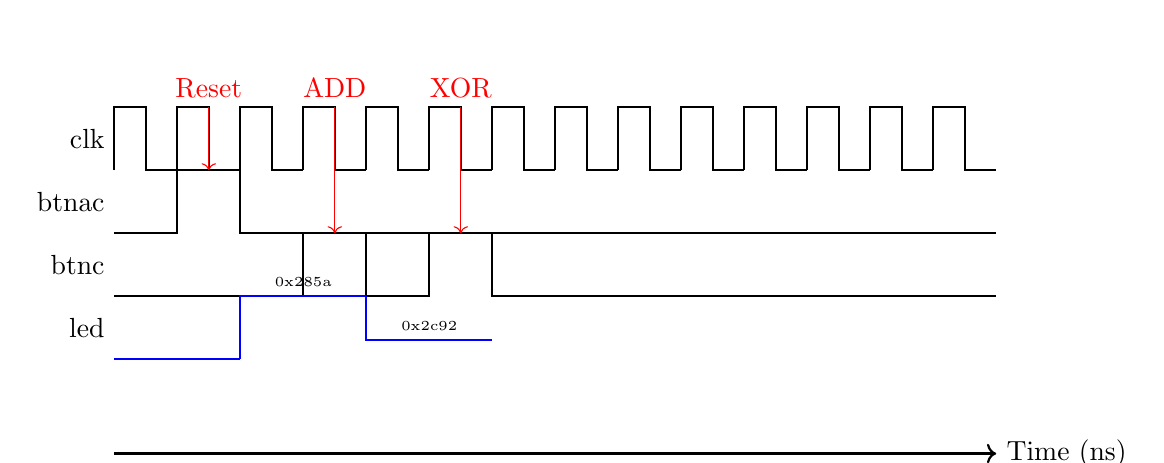
\begin{tikzpicture}[scale=0.8]
    % Time axis
    \draw[->,thick] (0,0) -- (14,0) node[right] {Time (ns)};
    
    % Clock
    \node[left] at (0,5) {clk};
    \foreach \i in {0,1,2,3,4,5,6,7,8,9,10,11,12,13} {
        \draw[thick] (\i,4.5) -- (\i,5.5) -- (\i+0.5,5.5) -- (\i+0.5,4.5) -- (\i+1,4.5);
    }
    
    % btnac
    \node[left] at (0,4) {btnac};
    \draw[thick] (0,3.5) -- (1,3.5) -- (1,4.5) -- (2,4.5) -- (2,3.5) -- (14,3.5);
    
    % btnc
    \node[left] at (0,3) {btnc};
    \draw[thick] (0,2.5) -- (3,2.5) -- (3,3.5) -- (4,3.5) -- (4,2.5) -- 
                 (5,2.5) -- (5,3.5) -- (6,3.5) -- (6,2.5) -- (14,2.5);
    
    % led
    \node[left] at (0,2) {led};
    \draw[thick,blue] (0,1.5) -- (2,1.5);
    \draw[thick,blue] (2,1.5) -- (2,2.5) -- (4,2.5);
    \node[above,font=\tiny] at (3,2.5) {0x285a};
    \draw[thick,blue] (4,2.5) -- (4,1.8) -- (6,1.8);
    \node[above,font=\tiny] at (5,1.8) {0x2c92};
    
    % Annotations
    \draw[<-,red] (1.5,4.5) -- (1.5,5.5) node[above] {Reset};
    \draw[<-,red] (3.5,3.5) -- (3.5,5.5) node[above] {ADD};
    \draw[<-,red] (5.5,3.5) -- (5.5,5.5) node[above] {XOR};
\end{tikzpicture}
\caption{Σχηματική αναπαράσταση κυματομορφών αριθμομηχανής}
\end{figure}

\textbf{Σημείωση:} Για λεπτομερείς κυματομορφές, χρησιμοποιήστε τα αρχεία VCD που παράγονται από τα testbenches στο Playground EDA.

\subsection{Κυματομορφές Νευρωνικού (Άσκηση 4)}

\begin{figure}[H]
\centering
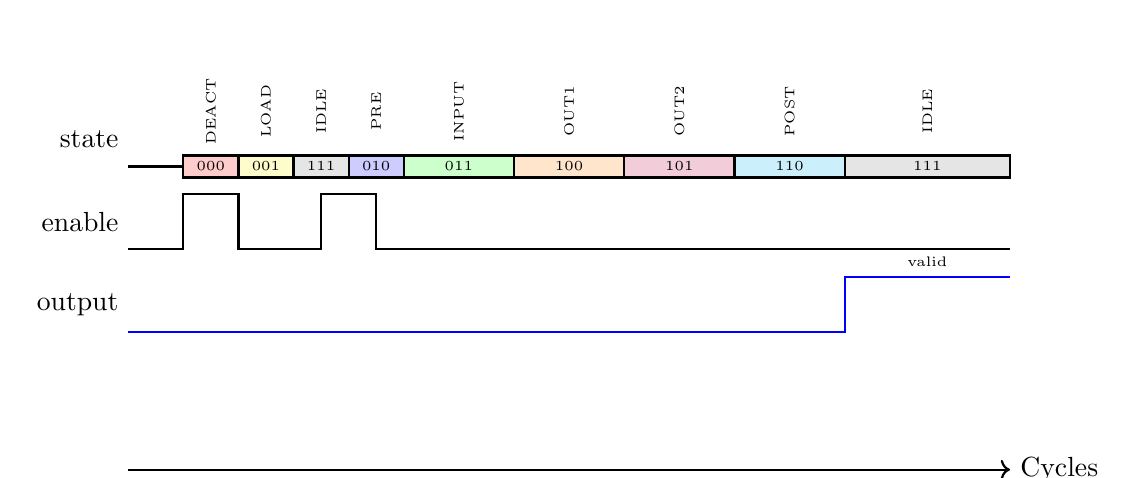
\begin{tikzpicture}[scale=0.7]
    % Time axis
    \draw[->,thick] (0,0) -- (16,0) node[right] {Cycles};
    
    % FSM State
    \node[left] at (0,6) {state};
    \draw[thick] (0,5.5) -- (1,5.5);
    \draw[thick,fill=red!20] (1,5.3) rectangle (2,5.7);
    \node[font=\tiny] at (1.5,5.5) {000};
    \draw[thick,fill=yellow!20] (2,5.3) rectangle (3,5.7);
    \node[font=\tiny] at (2.5,5.5) {001};
    \draw[thick,fill=gray!20] (3,5.3) rectangle (4,5.7);
    \node[font=\tiny] at (3.5,5.5) {111};
    \draw[thick,fill=blue!20] (4,5.3) rectangle (5,5.7);
    \node[font=\tiny] at (4.5,5.5) {010};
    \draw[thick,fill=green!20] (5,5.3) rectangle (7,5.7);
    \node[font=\tiny] at (6,5.5) {011};
    \draw[thick,fill=orange!20] (7,5.3) rectangle (9,5.7);
    \node[font=\tiny] at (8,5.5) {100};
    \draw[thick,fill=purple!20] (9,5.3) rectangle (11,5.7);
    \node[font=\tiny] at (10,5.5) {101};
    \draw[thick,fill=cyan!20] (11,5.3) rectangle (13,5.7);
    \node[font=\tiny] at (12,5.5) {110};
    \draw[thick,fill=gray!20] (13,5.3) rectangle (16,5.7);
    \node[font=\tiny] at (14.5,5.5) {111};
    
    % Enable
    \node[left] at (0,4.5) {enable};
    \draw[thick] (0,4) -- (1,4) -- (1,5) -- (2,5) -- (2,4) --
                 (3.5,4) -- (3.5,5) -- (4.5,5) -- (4.5,4) -- (16,4);
    
    % final_output
    \node[left] at (0,3) {output};
    \draw[thick,blue] (0,2.5) -- (13,2.5) -- (13,3.5) -- (16,3.5);
    \node[above,font=\tiny] at (14.5,3.5) {valid};
    
    % Annotations
    \node[font=\tiny,rotate=90] at (1.5,6.5) {DEACT};
    \node[font=\tiny,rotate=90] at (2.5,6.5) {LOAD};
    \node[font=\tiny,rotate=90] at (3.5,6.5) {IDLE};
    \node[font=\tiny,rotate=90] at (4.5,6.5) {PRE};
    \node[font=\tiny,rotate=90] at (6,6.5) {INPUT};
    \node[font=\tiny,rotate=90] at (8,6.5) {OUT1};
    \node[font=\tiny,rotate=90] at (10,6.5) {OUT2};
    \node[font=\tiny,rotate=90] at (12,6.5) {POST};
    \node[font=\tiny,rotate=90] at (14.5,6.5) {IDLE};
\end{tikzpicture}
\caption{Σχηματική αναπαράσταση κυματομορφών FSM νευρωνικού}
\end{figure}

%==============================================================================
\section{Συμπεράσματα}
%==============================================================================

Η εργασία ολοκληρώθηκε επιτυχώς με τα ακόλουθα αποτελέσματα:

\begin{enumerate}
    \item \textbf{ALU (alu.v):} Υλοποιήθηκε 32-bit ALU με 12 λειτουργίες και ανίχνευση υπερχείλισης
    \item \textbf{Αριθμομηχανή (calc.v, calc\_enc.v):} Λειτουργική αριθμομηχανή με structural encoder βασισμένο στα σχήματα της εκφώνησης
    \item \textbf{Register File (regfile.v):} 16×32-bit με σύγχρονη ανάγνωση (ένα always block) και data forwarding
    \item \textbf{Νευρωνικό (mac\_unit.v, nn.v):} \textbf{Moore FSM} για ασφάλεια και συγχρονισμό, τεχνική pre-fetching για το Register File, και χειρισμό overflow
\end{enumerate}

\textbf{Βασικές Σχεδιαστικές Αποφάσεις:}
\begin{itemize}
    \item Επιλογή \textbf{Moore FSM} αντί Mealy για καθαρό συγχρονισμό και αποφυγή glitches
    \item Υλοποίηση \textbf{σύγχρονης ανάγνωσης} στο Register File όπως ζητούσε η εκφώνηση, με τεχνική pre-fetching στο FSM
    \item Διαχωρισμός του output layer σε 2 καταστάσεις (S5a, S5b) για αποφυγή combinatorial loop
    \item Προσαρμογή της τιμής overflow σε \texttt{0xFFFFFFFF} για συμβατότητα με το \texttt{nn\_model.v}
\end{itemize}

Τα testbenches επιβεβαίωσαν την ορθή λειτουργία όλων των κυκλωμάτων. Η προσομοίωση πραγματοποιήθηκε στο EDA Playground με Icarus Verilog 12.

%==============================================================================
\section{Αναφορές}
%==============================================================================

\begin{enumerate}
    \item Ψηφιακή Σχεδίαση, 6η Έκδοση, Morris Mano and Michael Ciletti
    \item IEEE Standard for Verilog Hardware Description Language (IEEE 1364-2005)
    \item Playground EDA - Online Verilog Simulator \url{https://eda-playground.readthedocs.io/}
\end{enumerate}

%==============================================================================
\section*{Παράρτημα: Λίστα Αρχείων}
%==============================================================================

\begin{table}[H]
\centering
\begin{tabular}{|l|l|}
\hline
\textbf{Αρχείο} & \textbf{Περιγραφή} \\
\hline
alu.v & Αριθμητική/Λογική Μονάδα 32-bit \\
calc.v & Module αριθμομηχανής \\
calc\_enc.v & Encoder για alu\_op (structural) \\
calc\_tb.v & Testbench αριθμομηχανής \\
regfile.v & Register File 16×32-bit \\
mac\_unit.v & Multiply-Accumulate Unit \\
nn.v & Νευρωνικό δίκτυο με FSM \\
tb\_nn.v & Testbench νευρωνικού \\
\hline
\end{tabular}
\caption{Λίστα αρχείων εργασίας}
\end{table}

\end{document}